\documentclass[varwidth]{standalone}
\usepackage{tikz}
\begin{document}
    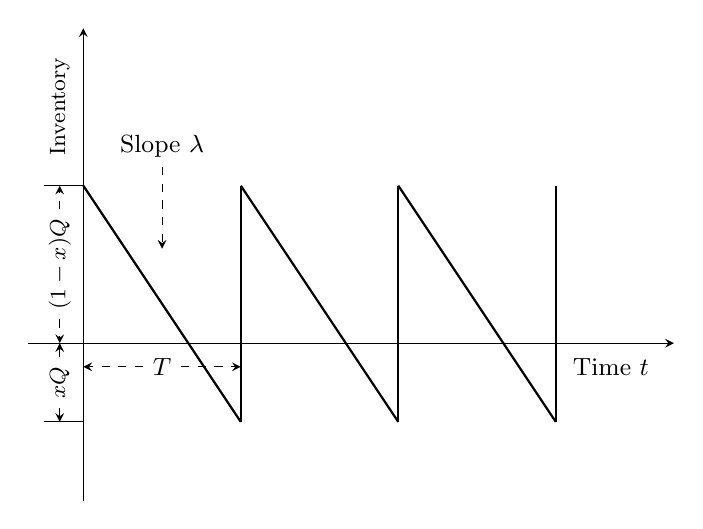
\begin{tikzpicture}
        [
            Axis/.style={-stealth},
            Plot/.style={thick},
            Fill/.style={fill=grey!20},
            Notation/.style={dashed, -stealth},
            VLabel/.style={rotate=90, font=\footnotesize},
            HLabel/.style={font=\small}
        ]
        \draw[Axis] (-0.7, 0) -- (7.5, 0);
        \draw[Axis] (0, -2) -- (0, 4);
        \foreach \x in {1, 2, 3} {
            \draw[Plot] (2 * \x - 2, 2) -- (2 * \x, -1);
            \draw[Plot] (2 * \x, -1) -- (2 * \x, 2);
        }
        \draw (2, -0.5) -- (2, 0);
        \draw (-0.5, 2) -- (0, 2);
        \draw (-0.5, -1) -- (0, -1);
        \node[HLabel] (Label_T) at (1, -0.3) {$T$};
        \draw[Notation] (Label_T) -> (0, -0.3);
        \draw[Notation] (Label_T) -> (2, -0.3);
        \node[VLabel] (Label_Qp) at (-0.3, 1) {$(1-x)Q$};
        \draw[Notation] (Label_Qp) -> (-0.3, 0);
        \draw[Notation] (Label_Qp) -> (-0.3, 2);
        \node[VLabel] (Label_Qm) at (-0.3, -0.5) {$xQ$};
        \draw[Notation] (Label_Qm) -> (-0.3, 0);
        \draw[Notation] (Label_Qm) -> (-0.3, -1);
        \node[HLabel] (XLabel) at (6.7, -0.3) {Time $t$};
        \node[VLabel] (YLabel) at (-0.3, 3) {Inventory};

        \node[HLabel] (Slope) at (1, 2.5) {Slope $\lambda$};
        \draw[Notation] (Slope) -> (1, 1.2);
    \end{tikzpicture}
\end{document}